\chapter{The working process}
Since this project can be seen as the development of a professional software system, intended for use by someone other than the developer, rather than personal software development and usage, it can be considered software engineering\cite{sommerville9ed}. As the developers on this project is a group of students, together a team, and a professional software system is usually developed in teams, this project could get support from various software engineering techniques.

In software engineering two types of software planning are usually relevant\cite{sommerville9ed} Plan-driven and agile. In the plan-driven process all activities are planned in advance, and progress is measured against this plan\cite{sommerville9ed}. The agile process is incremental, and it is easier to return to previous activities and make changes, for instance a change in requirements and the impact it has on elements based thereof.

\begin{figure}[h!]
\centering
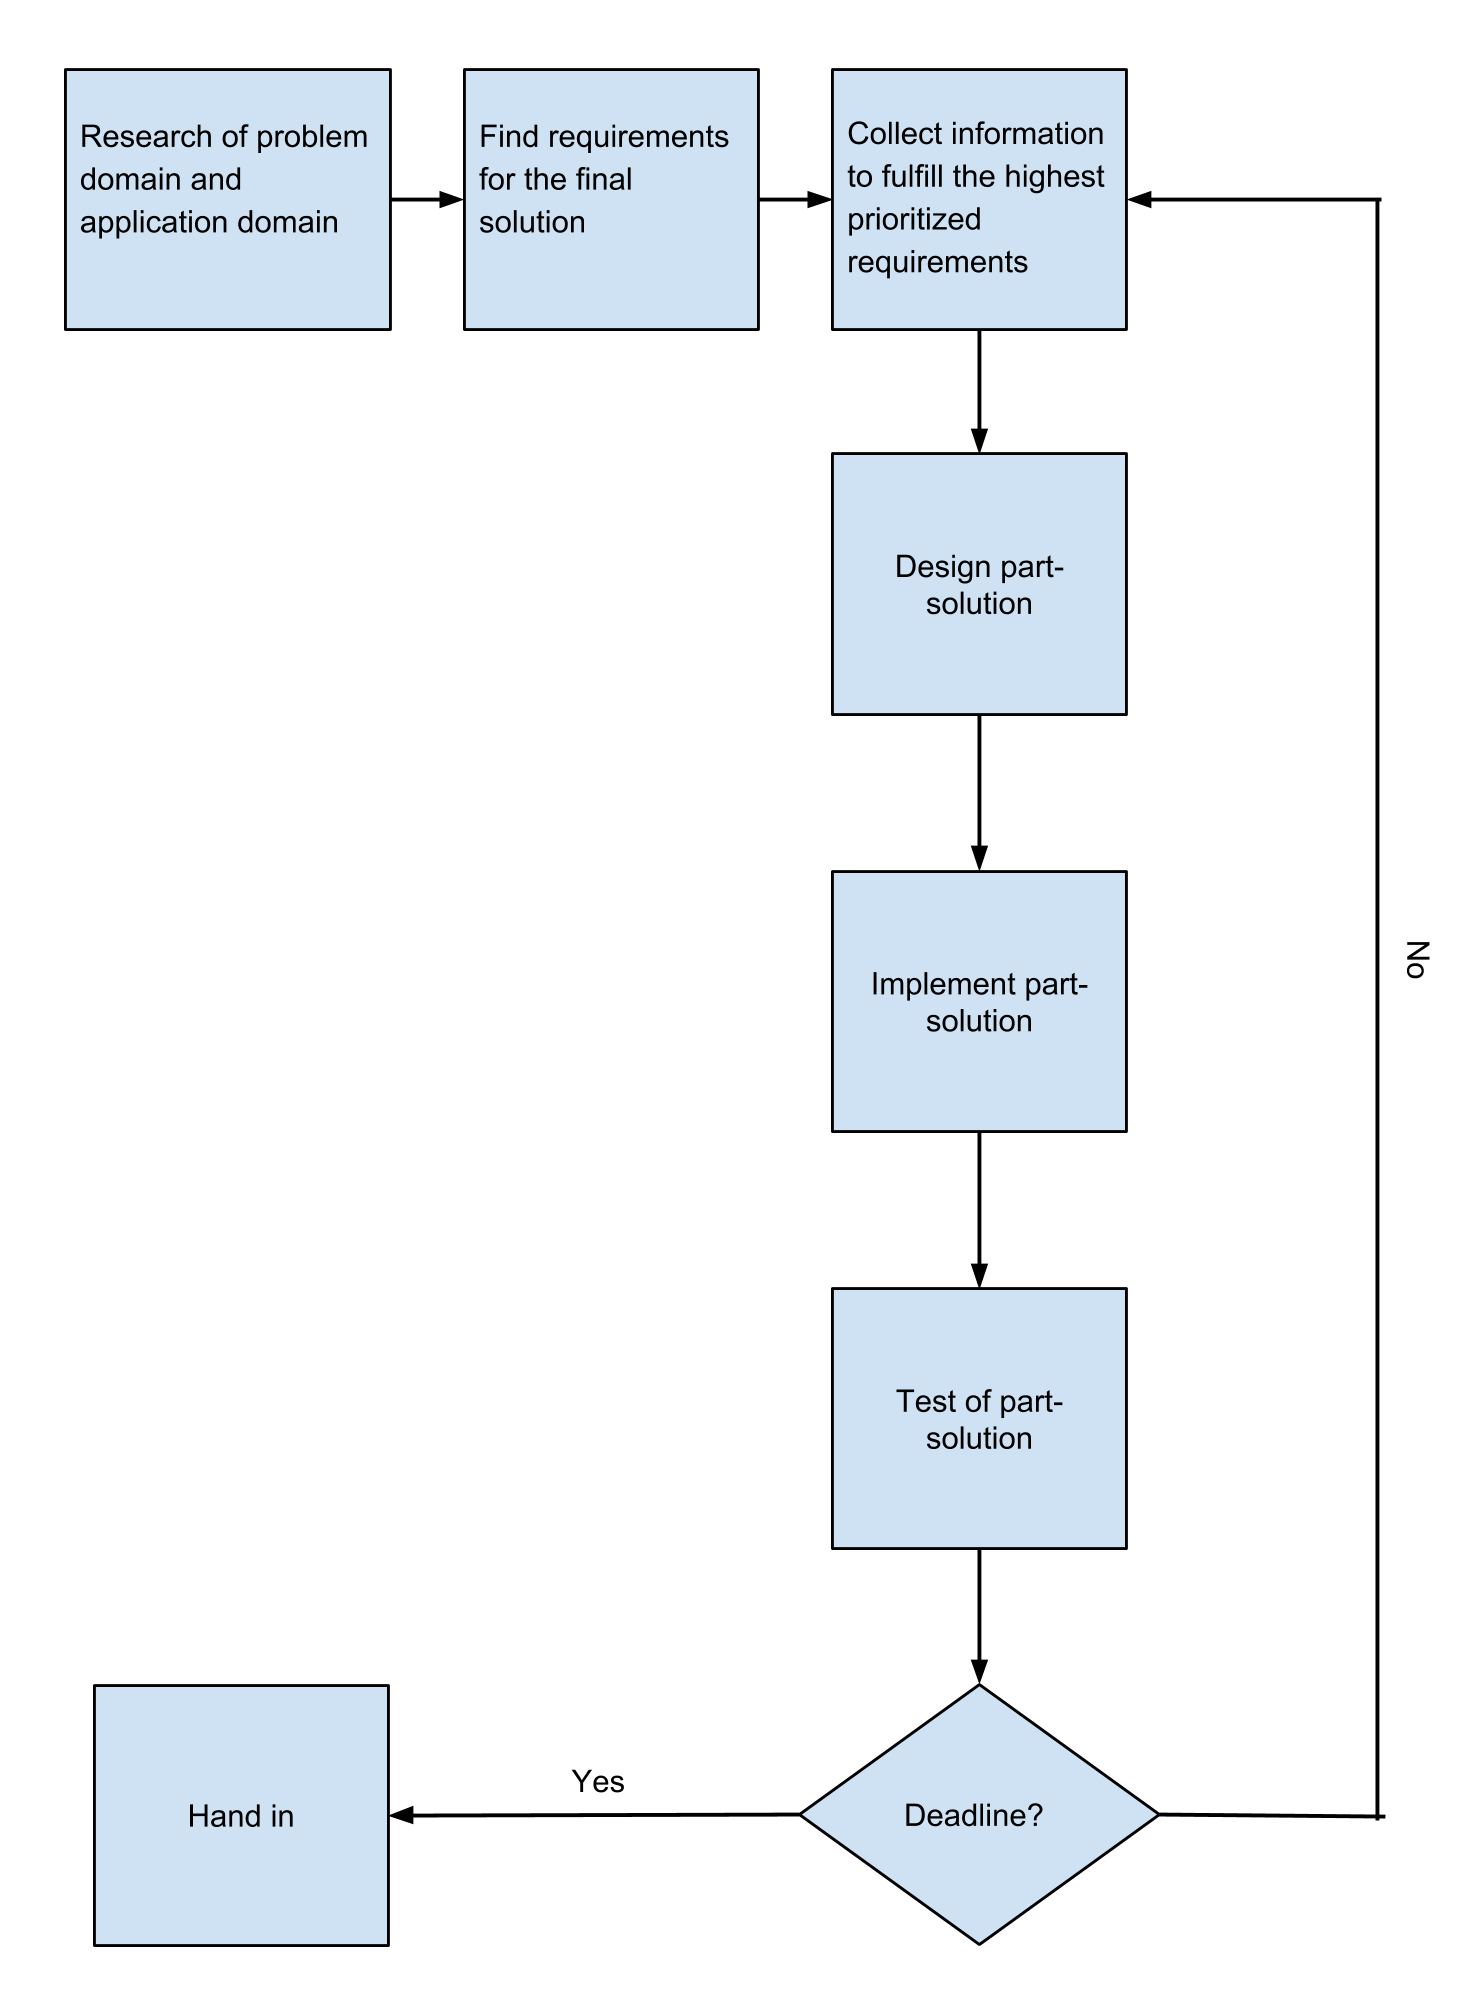
\includegraphics[width=1.2\textwidth]{figures/ProcessmodelDiagram.png}
\caption{Process model diagram.}
\label{fig:processmodelDiagram}
\end{figure}

The flow chart in \figref{processmodelDiagram} shows this project's process model and displays the different stages of the project. This process model is a mix between the plan-driven and the agile method, but they are separated to different areas of the developing process. The project initializes in a plan-driven manner, while the implementation part is done in an agile manner.

The plan-driven part consist of the two first stages of the project. First the problem domain and application domain will be researched and analyzed. This enables the construction of requirements for the solution to be developed. The requirement is assumed not to change during the project period. In the next stage the requirements will be given priorities in order to determine the their importance for the final solution. The priorities are given by performing a MoSCoW analysis.

The next four stages are performed in an agile manner. Whenever the last of the four stages have been completed, which is the test stage, the time left until deadline is evaluated. If there is enough time left, then the four agile stages will be repeated. This is where the priorities that was given during the MoSCoW analysis becomes relevant. Each iteration will focus on a single tier of the requirements e.g. first iteration will focus on the "Must have" requirements. These will be the requirements in focus. If these requirements are considered met at the end of the four stages, then the next iteration will focus on the next tier of requirements, which in this example would be "Should have" priorities.

Research on how to meet the requirements in focus is done during the first stage of the agile stage followed by the second stage where the design of the solution will be developed. The designed solution will in the third stage be implemented.

The solution will be tested as a follow up to the implementation. Here it will be determined whether the requirements in focus are met. If the requirements were not met, then the requirements in focus will remain during the next iteration. If the requirements are met, then the next iteration will focus on the next tier of requirements. An extra iteration will only be considered if there is sufficient time left until the deadline.

An agile implementation process is chosen, because the domain of the project is new and unknown for all group members, and therefore hard to plan considering time. Furthermore, this project has an impassable deadline, and therefore it would be hard for the group to set up a perfect set of requirements that would correspond to the project timespan. Keeping focus on a single tier at the time ensures that the most important features of the requirements are met first, which can then be expanded upon.
































